%% Copyright 2005 G. W. Knor
%%This work may be distributed and/or modified under the
% conditions of the LaTeX Project Public License, either version 1.3
% of this license or (at your option) any later version.
% The latest version of this license is in
% http://www.latex-project.org/lppl.txt
% and version 1.3 or later is part of all distributions of LaTeX
% version 2005/12/01 or later.
%%This work has the LPPL maintenance status "maintained".
%%The Current Maintainer of this work is G. W. Knor.

\documentclass{beamer}
\usepackage{graphicx}
\usepackage{amsmath} % provides \text{<stuff>} which prints <stuff> in text mode
\usepackage{sidecap}
\usepackage{courier}
\usepackage{listings}
\usepackage{hyperref}
\usepackage[utf8]
{inputenc}
\lstset{
    breaklines=true,
    breakatwhitespace=true,
    postbreak=\raisebox{0ex}[0ex][0ex]{
        \ensuremath{
            \color{red}\hookrightarrow\space
        }
    }
}
\setcounter{tocdepth}{1}

\definecolor{keywords}{RGB}{255,0,90}
\definecolor{comments}{RGB}{0,0,113}
\definecolor{red}{RGB}{160,0,0}
\definecolor{green}{RGB}{0,150,0}

\lstset{
    language=Python,
    basicstyle=\ttfamily\footnotesize,
    keywordstyle=\color{keywords},
    commentstyle=\color{comments},
    stringstyle=\color{red},
    showstringspaces=false,
    identifierstyle=\color{green}
}


\title{HowTo re}
\author{Dariusz Śmigiel}
\date{PyCon PL 2015}
\usetheme{Warsaw}
\usecolortheme{beaver}

\begin{document}

\begin{frame}
\titlepage
\end{frame}

\section{History}
\subsection{Origins}
\begin{frame}
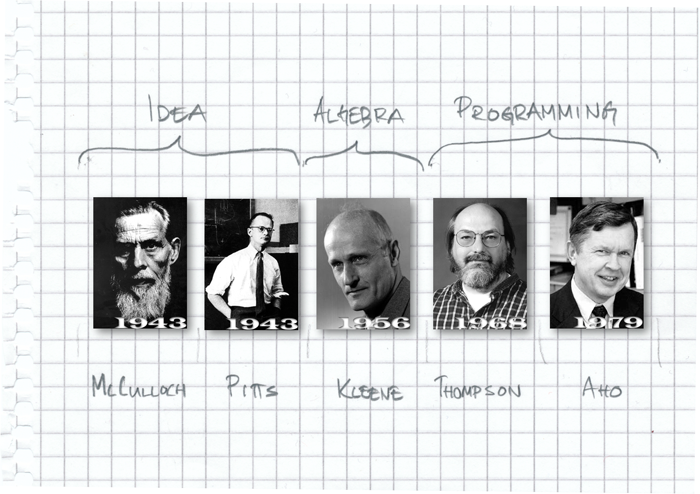
\includegraphics[width=1\textwidth]{images/history.png}
\end{frame}

\subsection{re module}
\begin{frame}
Delivering Quality since December 31, 1997 \\
\pause
Release of Python 1.5
\pause

\begin{itemize}
 \item Deprecated old module `regex`, based on Perl-style patterns.
\pause
 \item `regex` finally removed in Python 2.5.
\end{itemize}
\end{frame}

\section{Do I need it?}
\subsection{Matching / Modifying}
\begin{frame}
Answer for questions:
 \begin{itemize}
  \item "Does this string match the pattern?"
  \item "Is there a match for the pattern anywhere in this string?"
 \end{itemize}
 \pause
 \begin{itemize}
  \item Replace part of it
  \item Split into pieces
 \end{itemize}
\end{frame}

\section{Under the hood}
\subsection{Implementation / Features}
\begin{frame}[fragile]
 re is handled as string  - there is no special syntax for expressing it (advantage and disadvantage) \\
 \pause
 re patterns are compiled into bytecode \\
 \pause
 re module is a C extension module (like \verb/socket/ or \verb/zlib/) \\
 \pause
 re language is relatively small and restricted
 \pause
 \begin{itemize}
  \item not all possible string processing tasks can be done
  \item some of them can be done, but expression would be very complicated
 \end{itemize}
\end{frame}

\subsection{Regex Example}
\begin{frame}[fragile]
\begingroup
 \fontsize{6pt}{8pt}\selectfont
\begin{verbatim}
(?:(?:\r\n)?[ \t])*(?:(?:(?:[^()<>@,;:\\".\[\] \000-\031]+(?:(?:(?:\r\n)?[ \t]
)+|\Z|(?=[\["()<>@,;:\\".\[\]]))|"(?:[^\"\r\\]|\\.|(?:(?:\r\n)?[ \t]))*"(?:(?:
\r\n)?[ \t])*)(?:\.(?:(?:\r\n)?[ \t])*(?:[^()<>@,;:\\".\[\] \000-\031]+(?:(?:(
?:\r\n)?[ \t])+|\Z|(?=[\["()<>@,;:\\".\[\]]))|"(?:[^\"\r\\]|\\.|(?:(?:\r\n)?[
\t]))*"(?:(?:\r\n)?[ \t])*))*@(?:(?:\r\n)?[ \t])*(?:[^()<>@,;:\\".\[\] \000-\0
31]+(?:(?:(?:\r\n)?[ \t])+|\Z|(?=[\["()<>@,;:\\".\[\]]))|\[([^\[\]\r\\]|\\.)*\
](?:(?:\r\n)?[ \t])*)(?:\.(?:(?:\r\n)?[ \t])*(?:[^()<>@,;:\\".\[\] \000-\031]+
(?:(?:(?:\r\n)?[ \t])+|\Z|(?=[\["()<>@,;:\\".\[\]]))|\[([^\[\]\r\\]|\\.)*\](?:
(?:\r\n)?[ \t])*))*|(?:[^()<>@,;:\\".\[\] \000-\031]+(?:(?:(?:\r\n)?[ \t])+|\Z
|(?=[\["()<>@,;:\\".\[\]]))|"(?:[^\"\r\\]|\\.|(?:(?:\r\n)?[ \t]))*"(?:(?:\r\n)
?[ \t])*)*\<(?:(?:\r\n)?[ \t])*(?:@(?:[^()<>@,;:\\".\[\] \000-\031]+(?:(?:(?:\
r\n)?[ \t])+|\Z|(?=[\["()<>@,;:\\".\[\]]))|\[([^\[\]\r\\]|\\.)*\](?:(?:\r\n)?[
 \t])*)(?:\.(?:(?:\r\n)?[ \t])*(?:[^()<>@,;:\\".\[\] \000-\031]+(?:(?:(?:\r\n)
?[ \t])+|\Z|(?=[\["()<>@,;:\\".\[\]]))|\[([^\[\]\r\\]|\\.)*\](?:(?:\r\n)?[ \t]
)*))*(?:,@(?:(?:\r\n)?[ \t])*(?:[^()<>@,;:\\".\[\] \000-\031]+(?:(?:(?:\r\n)?[
 \t])+|\Z|(?=[\["()<>@,;:\\".\[\]]))|\[([^\[\]\r\\]|\\.)*\](?:(?:\r\n)?[ \t])*
)(?:\.(?:(?:\r\n)?[ \t])*(?:[^()<>@,;:\\".\[\] \000-\031]+(?:(?:(?:\r\n)?[ \t]
)+|\Z|(?=[\["()<>@,;:\\".\[\]]))|\[([^\[\]\r\\]|\\.)*\](?:(?:\r\n)?[ \t])*))*)
*:(?:(?:\r\n)?[ \t])*)?(?:[^()<>@,;:\\".\[\] \000-\031]+(?:(?:(?:\r\n)?[ \t])+
|\Z|(?=[\["()<>@,;:\\".\[\]]))|"(?:[^\"\r\\]|\\.|(?:(?:\r\n)?[ \t]))*"(?:(?:\r
\n)?[ \t])*)(?:\.(?:(?:\r\n)?[ \t])*(?:[^()<>@,;:\\".\[\] \000-\031]+(?:(?:(?:
\end{verbatim}
 \endgroup
\end{frame}

\begin{frame}[fragile]
\begingroup
 \fontsize{6pt}{8pt}\selectfont
\begin{verbatim}
\r\n)?[ \t])+|\Z|(?=[\["()<>@,;:\\".\[\]]))|"(?:[^\"\r\\]|\\.|(?:(?:\r\n)?[ \t
]))*"(?:(?:\r\n)?[ \t])*))*@(?:(?:\r\n)?[ \t])*(?:[^()<>@,;:\\".\[\] \000-\031
]+(?:(?:(?:\r\n)?[ \t])+|\Z|(?=[\["()<>@,;:\\".\[\]]))|\[([^\[\]\r\\]|\\.)*\](
?:(?:\r\n)?[ \t])*)(?:\.(?:(?:\r\n)?[ \t])*(?:[^()<>@,;:\\".\[\] \000-\031]+(?
:(?:(?:\r\n)?[ \t])+|\Z|(?=[\["()<>@,;:\\".\[\]]))|\[([^\[\]\r\\]|\\.)*\](?:(?
:\r\n)?[ \t])*))*\>(?:(?:\r\n)?[ \t])*)|(?:[^()<>@,;:\\".\[\] \000-\031]+(?:(?
:(?:\r\n)?[ \t])+|\Z|(?=[\["()<>@,;:\\".\[\]]))|"(?:[^\"\r\\]|\\.|(?:(?:\r\n)?
[ \t]))*"(?:(?:\r\n)?[ \t])*)*:(?:(?:\r\n)?[ \t])*(?:(?:(?:[^()<>@,;:\\".\[\]
\000-\031]+(?:(?:(?:\r\n)?[ \t])+|\Z|(?=[\["()<>@,;:\\".\[\]]))|"(?:[^\"\r\\]|
\\.|(?:(?:\r\n)?[ \t]))*"(?:(?:\r\n)?[ \t])*)(?:\.(?:(?:\r\n)?[ \t])*(?:[^()<>
@,;:\\".\[\] \000-\031]+(?:(?:(?:\r\n)?[ \t])+|\Z|(?=[\["()<>@,;:\\".\[\]]))|"
(?:[^\"\r\\]|\\.|(?:(?:\r\n)?[ \t]))*"(?:(?:\r\n)?[ \t])*))*@(?:(?:\r\n)?[ \t]
)*(?:[^()<>@,;:\\".\[\] \000-\031]+(?:(?:(?:\r\n)?[ \t])+|\Z|(?=[\["()<>@,;:\\
".\[\]]))|\[([^\[\]\r\\]|\\.)*\](?:(?:\r\n)?[ \t])*)(?:\.(?:(?:\r\n)?[ \t])*(?
:[^()<>@,;:\\".\[\] \000-\031]+(?:(?:(?:\r\n)?[ \t])+|\Z|(?=[\["()<>@,;:\\".\[
\]]))|\[([^\[\]\r\\]|\\.)*\](?:(?:\r\n)?[ \t])*))*|(?:[^()<>@,;:\\".\[\] \000-
\031]+(?:(?:(?:\r\n)?[ \t])+|\Z|(?=[\["()<>@,;:\\".\[\]]))|"(?:[^\"\r\\]|\\.|(
?:(?:\r\n)?[ \t]))*"(?:(?:\r\n)?[ \t])*)*\<(?:(?:\r\n)?[ \t])*(?:@(?:[^()<>@,;
:\\".\[\] \000-\031]+(?:(?:(?:\r\n)?[ \t])+|\Z|(?=[\["()<>@,;:\\".\[\]]))|\[([
^\[\]\r\\]|\\.)*\](?:(?:\r\n)?[ \t])*)(?:\.(?:(?:\r\n)?[ \t])*(?:[^()<>@,;:\\"
.\[\] \000-\031]+(?:(?:(?:\r\n)?[ \t])+|\Z|(?=[\["()<>@,;:\\".\[\]]))|\[([^\[\
\end{verbatim}
 \endgroup
\end{frame}

\begin{frame}[fragile]
\begingroup
 \fontsize{6pt}{8pt}\selectfont
\begin{verbatim}
]\r\\]|\\.)*\](?:(?:\r\n)?[ \t])*))*(?:,@(?:(?:\r\n)?[ \t])*(?:[^()<>@,;:\\".\
[\] \000-\031]+(?:(?:(?:\r\n)?[ \t])+|\Z|(?=[\["()<>@,;:\\".\[\]]))|\[([^\[\]\
r\\]|\\.)*\](?:(?:\r\n)?[ \t])*)(?:\.(?:(?:\r\n)?[ \t])*(?:[^()<>@,;:\\".\[\]
\000-\031]+(?:(?:(?:\r\n)?[ \t])+|\Z|(?=[\["()<>@,;:\\".\[\]]))|\[([^\[\]\r\\]
|\\.)*\](?:(?:\r\n)?[ \t])*))*)*:(?:(?:\r\n)?[ \t])*)?(?:[^()<>@,;:\\".\[\] \0
00-\031]+(?:(?:(?:\r\n)?[ \t])+|\Z|(?=[\["()<>@,;:\\".\[\]]))|"(?:[^\"\r\\]|\\
.|(?:(?:\r\n)?[ \t]))*"(?:(?:\r\n)?[ \t])*)(?:\.(?:(?:\r\n)?[ \t])*(?:[^()<>@,
;:\\".\[\] \000-\031]+(?:(?:(?:\r\n)?[ \t])+|\Z|(?=[\["()<>@,;:\\".\[\]]))|"(?
:[^\"\r\\]|\\.|(?:(?:\r\n)?[ \t]))*"(?:(?:\r\n)?[ \t])*))*@(?:(?:\r\n)?[ \t])*
(?:[^()<>@,;:\\".\[\] \000-\031]+(?:(?:(?:\r\n)?[ \t])+|\Z|(?=[\["()<>@,;:\\".
\[\]]))|\[([^\[\]\r\\]|\\.)*\](?:(?:\r\n)?[ \t])*)(?:\.(?:(?:\r\n)?[ \t])*(?:[
^()<>@,;:\\".\[\] \000-\031]+(?:(?:(?:\r\n)?[ \t])+|\Z|(?=[\["()<>@,;:\\".\[\]
]))|\[([^\[\]\r\\]|\\.)*\](?:(?:\r\n)?[ \t])*))*\>(?:(?:\r\n)?[ \t])*)(?:,\s*(
?:(?:[^()<>@,;:\\".\[\] \000-\031]+(?:(?:(?:\r\n)?[ \t])+|\Z|(?=[\["()<>@,;:\\
".\[\]]))|"(?:[^\"\r\\]|\\.|(?:(?:\r\n)?[ \t]))*"(?:(?:\r\n)?[ \t])*)(?:\.(?:(
?:\r\n)?[ \t])*(?:[^()<>@,;:\\".\[\] \000-\031]+(?:(?:(?:\r\n)?[ \t])+|\Z|(?=[
\["()<>@,;:\\".\[\]]))|"(?:[^\"\r\\]|\\.|(?:(?:\r\n)?[ \t]))*"(?:(?:\r\n)?[ \t
])*))*@(?:(?:\r\n)?[ \t])*(?:[^()<>@,;:\\".\[\] \000-\031]+(?:(?:(?:\r\n)?[ \t
])+|\Z|(?=[\["()<>@,;:\\".\[\]]))|\[([^\[\]\r\\]|\\.)*\](?:(?:\r\n)?[ \t])*)(?
:\.(?:(?:\r\n)?[ \t])*(?:[^()<>@,;:\\".\[\] \000-\031]+(?:(?:(?:\r\n)?[ \t])+|
\Z|(?=[\["()<>@,;:\\".\[\]]))|\[([^\[\]\r\\]|\\.)*\](?:(?:\r\n)?[ \t])*))*|(?:
\end{verbatim}
 \endgroup
\end{frame}

\begin{frame}[fragile]
\begingroup
 \fontsize{6pt}{8pt}\selectfont
\begin{verbatim}
[^()<>@,;:\\".\[\] \000-\031]+(?:(?:(?:\r\n)?[ \t])+|\Z|(?=[\["()<>@,;:\\".\[\
]]))|"(?:[^\"\r\\]|\\.|(?:(?:\r\n)?[ \t]))*"(?:(?:\r\n)?[ \t])*)*\<(?:(?:\r\n)
?[ \t])*(?:@(?:[^()<>@,;:\\".\[\] \000-\031]+(?:(?:(?:\r\n)?[ \t])+|\Z|(?=[\["
()<>@,;:\\".\[\]]))|\[([^\[\]\r\\]|\\.)*\](?:(?:\r\n)?[ \t])*)(?:\.(?:(?:\r\n)
?[ \t])*(?:[^()<>@,;:\\".\[\] \000-\031]+(?:(?:(?:\r\n)?[ \t])+|\Z|(?=[\["()<>
@,;:\\".\[\]]))|\[([^\[\]\r\\]|\\.)*\](?:(?:\r\n)?[ \t])*))*(?:,@(?:(?:\r\n)?[
 \t])*(?:[^()<>@,;:\\".\[\] \000-\031]+(?:(?:(?:\r\n)?[ \t])+|\Z|(?=[\["()<>@,
;:\\".\[\]]))|\[([^\[\]\r\\]|\\.)*\](?:(?:\r\n)?[ \t])*)(?:\.(?:(?:\r\n)?[ \t]
)*(?:[^()<>@,;:\\".\[\] \000-\031]+(?:(?:(?:\r\n)?[ \t])+|\Z|(?=[\["()<>@,;:\\
".\[\]]))|\[([^\[\]\r\\]|\\.)*\](?:(?:\r\n)?[ \t])*))*)*:(?:(?:\r\n)?[ \t])*)?
(?:[^()<>@,;:\\".\[\] \000-\031]+(?:(?:(?:\r\n)?[ \t])+|\Z|(?=[\["()<>@,;:\\".
\[\]]))|"(?:[^\"\r\\]|\\.|(?:(?:\r\n)?[ \t]))*"(?:(?:\r\n)?[ \t])*)(?:\.(?:(?:
\r\n)?[ \t])*(?:[^()<>@,;:\\".\[\] \000-\031]+(?:(?:(?:\r\n)?[ \t])+|\Z|(?=[\[
"()<>@,;:\\".\[\]]))|"(?:[^\"\r\\]|\\.|(?:(?:\r\n)?[ \t]))*"(?:(?:\r\n)?[ \t])
*))*@(?:(?:\r\n)?[ \t])*(?:[^()<>@,;:\\".\[\] \000-\031]+(?:(?:(?:\r\n)?[ \t])
+|\Z|(?=[\["()<>@,;:\\".\[\]]))|\[([^\[\]\r\\]|\\.)*\](?:(?:\r\n)?[ \t])*)(?:\
.(?:(?:\r\n)?[ \t])*(?:[^()<>@,;:\\".\[\] \000-\031]+(?:(?:(?:\r\n)?[ \t])+|\Z
|(?=[\["()<>@,;:\\".\[\]]))|\[([^\[\]\r\\]|\\.)*\](?:(?:\r\n)?[ \t])*))*\>(?:(
?:\r\n)?[ \t])*))*)?;\s*)
\end{verbatim}
 \endgroup
Perl regex to validate email addresses according to the RFC 822
\url{http://ex-parrot.com/~pdw/Mail-RFC822-Address}
\end{frame}

\section{Simple patterns}
\subsection{Metacharacters}
\begin{frame}[fragile]
\begin{verbatim}
. ^ $ * + ? { } [ ] \ | ( )
\end{verbatim}
\end{frame}

\subsubsection{Class}
\begin{frame}[fragile]
\verb/[ ]/ - class
\begin{lstlisting}
>>> import re
>>> re.findall("[def]", "abcdefghi")
['d', 'e', 'f']
>>> re.findall("[d-f]", "abcdefghi")
['d', 'e', 'f']
>>>
\end{lstlisting}
\pause
Metacharacters are not active inside class \\
\begin{lstlisting}
>>> re.findall("[d-f$]", "abcdefg$hi")
['d', 'e', 'f', '$']
\end{lstlisting}
\end{frame}

\subsubsection{Complementing set}
\begin{frame}[fragile]
\verb/^/ - complementing set
\begin{lstlisting}
>>> import re
>>> re.findall("[^5]", "abc 456 xyz")
['4', '6']
>>>
\end{lstlisting}
\end{frame}

\subsubsection{Dot - '.'}
\begin{frame}[fragile]
\verb/./ - dot. Matches anything except a newline character
\begin{lstlisting}
>>> import re
>>> regex = re.compile(".$")
>>> regex.findall("string")
['s', 't', 'r', 'i', 'n', 'g']
>>>
\end{lstlisting}
\pause
There is compilation flag, which changes default behavior.
\end{frame}

\subsection{Repeating Things}
\subsubsection{*, +, ?}
\begin{frame}[fragile]
\verb/*/ - star. Specifies that previous character can be matched zero or more times.
\begin{lstlisting}
>>> re.findall("ca*t", "ct, cat, caat")
['ct', 'cat', 'caat']
\end{lstlisting}
\pause
\verb/+/ - plus. Similar to \verb/*/, but requires at least one occurence of character.
\begin{lstlisting}
>>> re.findall("ca+t", "ct, cat, caat")
['cat', 'caat']
\end{lstlisting}
\pause
\verb/?/ - question mark. Matches either once or zero times
\begin{lstlisting}
>>> re.findall("ca?t", "ct, cat, caat")
['ct', 'cat']
\end{lstlisting}
\pause
\begin{lstlisting}
>>> re.findall("home-?brew", "homebrew, home-brew")
['homebrew', 'home-brew']
\end{lstlisting}
\end{frame}

\subsubsection{"{m,n}"}
\begin{frame}[fragile]
\verb/{m,n}/ - \verb/m/ and \verb/n/ are decimal numbers. There must be at least m repetitions, and at most n.
\begin{lstlisting}
>>> re.findall("a/{1,2}b", "ab, a/b, a//b, a///b")
['a/b', 'a//b']
\end{lstlisting}
\pause
\verb/m/ and \verb/n/ can be ommited. When m ommited, there is zero, when n ommited, upper bound infinity (more precisely, 2 billions)
\end{frame}

\subsection{Equivalents}
\begin{frame}[fragile]
\begin{verbatim}
{0,} == "*"
{1,} == "+"
{,1} == {0,1} == "?"
\end{verbatim}
\end{frame}

\subsection{Greedy}
\begin{frame}[fragile]
\verb/*/, \verb/+/ and \verb/?/ are greedy. Will try to repeat it as many times as possible (re engine can match only 2 billion characters (2GB) -- C \verb/int/ limitation). \\
\pause
\verb/a[bcd]*b/ - matches \verb/a/, zero or more letters from \verb/bcd/, and ends with \verb/b/ \\
\begin{center}
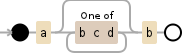
\includegraphics[width=0.5\textwidth]{images/greedy.png}
\end{center}
src: \url{https://www.debuggex.com/r/NT7_HIVhxI_h64zk}
\end{frame}

\begin{frame}[fragile]
\verb/abcbd/
\begin{itemize}
\item matches \verb/a/
\pause
\item matches \verb/abcbd/ to the end of the string
\pause
\item fails, because current position is the end of the string, so cannot match \verb/b/
\pause
\item matches \verb/abcb/ - one less character
\pause
\item fails, because current position is \verb/d/, so cannot match \verb/b/
\pause
\item matches \verb/abc/, so \verb/[bcd]*/ matches only \verb/bc/
\pause
\item \verb/abcb/, tries last character \verb/b/, and it's on current position
\pause
\item success
\end{itemize}
\begin{lstlisting}
>>> re.findall('a[bcd]*b', 'abcbd')
['abcb']
\end{lstlisting}
\end{frame}

\subsection{Non-greedy}
\begin{frame}[fragile]
\verb/*?, +?, ??, {m,n}?/ are non-greedy. Will try to match as few characters as possible.
\pause

\begin{lstlisting}
>>> import re
>>> text = "<html><head><title>Title</title></head></html>"
\end{lstlisting}
\pause
\begin{lstlisting}
>>> greedy_regex = re.compile("<.*>")
>>> greedy_regex.findall(text)
['<html><head><title>Title</title></head></html>']
\end{lstlisting}
\pause
\begin{lstlisting}
>>> non_greedy_regex = re.compile("<.*?>")
>>> non_greedy_regex.findall(text)
['<html>', '<head>', '<title>', '</title>', '</head>', '</html>']
>>>
\end{lstlisting}

\end{frame}

\subsection{Backslash - escape metacharacters}
\begin{frame}[fragile]
\verb/\/ - backslash (escape metacharacters) \\
For matching \verb/[/ or \verb/\/ you can use \verb/\[/ or \verb/\\/ \\
\begin{lstlisting}
>>> re.findall("\[\]", "Find brackets []")
['[]']
\end{lstlisting}
\pause
Some of special sequences beginning with \verb/\/ express predefined sets of characters: set of digits, letters, everything but whitespace
\end{frame}

\begin{frame}[fragile]
\begin{itemize}
\item \verb/\d/ - any decimal digit, equivalent of \verb/[0-9]/
\item \verb/\D/ - everything but decimal digit, equivalent of \verb/[^0-9]/
\end{itemize}
\begin{lstlisting}
>>> re.findall("\d", "abc789xyz")
['7', '8', '9']
>>> re.findall("[0-9]", "abc789xyz")
['7', '8', '9']
>>> re.findall("\D", "abc789xyz")
['a', 'b', 'c', 'x', 'y', 'z']
>>> re.findall("[^0-9]", "abc789xyz")
['a', 'b', 'c', 'x', 'y', 'z']
\end{lstlisting}
\end{frame}

\begin{frame}[fragile]
\begin{itemize}
\item \verb/\w/ - any alphanumeric: \verb/[a-zA-Z0-9_]/
\item \verb/\W/ - any non-alpahnumeric: \verb/[^a-zA-Z0-9_]/
\end{itemize}
\begin{lstlisting}
>>> re.findall('\w+', 'abc 789 xyz')
['abc', '789', 'xyz']
>>> re.findall('[a-zA-Z0-9_]+', 'abc 789 xyz')
['abc', '789', 'xyz']
>>> re.findall('\W+', 'abc 789 xyz')
[' ', ' ']
>>> re.findall('[^a-zA-Z0-9_]+', 'abc 789 xyz')
[' ', ' ']
\end{lstlisting}
\end{frame}

\begin{frame}[fragile]
\begin{itemize}
\item \verb/\s/ - any whitespace character: \verb/[ \t\n\r\f\v]/ \\ (space, tab (ASCII 0x09), newline (0x0A), return (0x0D), form feed - page break(0x0C), vertical tab (0x0B))
\item \verb/\S/ - any non-whitespace character: \verb/[^ \t\n\r\f\v]/
\pause
\item NOTE! Remember that Windows text files use \verb/\r\n/ to terminate lines, while UNIX text files use \verb/\n/.
\end{itemize}
\end{frame}

\begin{frame}[fragile]
\begin{lstlisting}
>>> text = "line,\nwith \ttab,\vvertical,\rreturn and \nnewlines."
>>> print(text)
line,
with    tab,
return and  vertical,
newlines.
>>> re.findall("\s+", text)
['\n', ' \t', '\x0b', '\r', ' ', ' \n']
>>> re.findall("[ \t\n\r\f\v]+", text)
['\n', ' \t', '\x0b', '\r', ' ', ' \n']
>>> re.findall("\S+", text)
['line,', 'with', 'tab,', 'vertical,', 'return', 'and', 'newlines.']
>>> re.findall("[^ \t\n\r\f\v]+", text)
['line,', 'with', 'tab,', 'vertical,', 'return', 'and', 'newlines.']
\end{lstlisting}
\end{frame}

\subsection{"Backslash Plague" problem}
\begin{frame}[fragile]
\begin{itemize}
\item re is handled as string
\item one of \verb/re/ metacharacters is \verb/\/
\item backslash for escaping in \verb/re/ conflicts with the same purpose in Python
\end{itemize}
\end{frame}

\begin{frame}[fragile]
\begin{tabular}{ | l | p{7cm} |}
\hline
Characters & Stage \\ \hline
\verb/\section/ & Text string to be matched \\
\verb/\\section/ & Escaped backslash for \verb/re.compile()/ \\
\verb/"\\\\section"/ & Escaped backslashes for a string literal \\
\hline
\end{tabular}
\pause
re string needs to be written as \verb/"\\\\"/ because regular expression must be \verb/\\/ and each must be escaped \verb/\\/ inside a regular Python string literal. \\
\pause
Solution - raw string
\begin{tabular}{ | l | p{7cm} |}
\hline
Regular string & Raw string \\ \hline
\verb/"ab*"/ & \verb/r"ab*"/ \\
\verb/"\\\\section"/ & \verb/r"\\section"/ \\
\verb/"\\w+\\s+"/ & \verb/r"\w+\s+"/ \\
\hline
\end{tabular}
\end{frame}

\begin{frame}[fragile]
\begin{lstlisting}
>>> latex = """
... \begin{document}
... \section{History}
... \subsection{Origins}
... \begin{frame}
... Content
... \end{frame}
... \end{document}
... """
>>> latex
'\n\x08egin{document}\n\\section{History}\n\\subsection{Origins}\n\x08egin{frame}\nContent\n\\end{frame}\n\\end{document}\n'
>>> re.findall(r"\\section", latex)
['\\section']
>>> print(re.findall(r"\\section{.*}", latex))
['\\section{History}']
>>> print(re.findall(r"\\section{.*}", latex)[0])
\section{History}
\end{lstlisting}
\end{frame}

\section{Regular Expressions}
\subsection{Compilation}
\begin{frame}[fragile]
\begin{lstlisting}
>>> import re
>>> regex = re.compile('[a-zA-Z0-9]+')
>>> regex
re.compile('[a-zA-Z0-9]+')
>>> regex.findall('Search test 01')
['Search', 'test', '01']
\end{lstlisting}
\pause
\begin{lstlisting}
>>> import re
>>> regex = re.compile('[a-zA-Z0-9]+')
>>> regex
re.compile('[a-zA-Z0-9]+')
>>> re.findall(regex, 'Search test 02')
['Search', 'test', '02']
\end{lstlisting}
\pause
\begin{lstlisting}
>>> import re
>>> re.findall('[a-zA-Z0-9]+', 'Search test 03')
['Search', 'test', '03']
\end{lstlisting}
\end{frame}

\subsection{Compilation Flags}
\subsubsection{re.DEBUG}
\begin{frame}[fragile]
\verb/re.DEBUG/
\begin{lstlisting}
>>> import re
>>> regex = re.compile('[a-z]', re.DEBUG)
in
  range (97, 122)
>>>
\end{lstlisting}
\end{frame}

\subsubsection{re.ASCII}
\begin{frame}[fragile]
\verb/re.ASCII, re.A/ \\
\verb/\xa0/ - non-breaking space
\begin{lstlisting}
>>> import re
>>> regex = re.compile("\s+")
>>> regex.findall("\xa0 ha")
['\xa0 ']
\end{lstlisting}
\pause
\begin{lstlisting}
>>> ascii_regex = re.compile("\s+", re.ASCII)
>>> ascii_regex.findall("\xa0 ha")
[' ']
>>>
\end{lstlisting}
\end{frame}

\subsubsection{re.IGNORECASE}
\begin{frame}[fragile]
\verb/re.IGNORECASE, re.I/ \\
\begin{lstlisting}
>>> import re
>>> text = "CamelCase CAPITAL and lower WoRd"
>>> regex = re.compile("[a-z]+")
>>> regex.findall(text)
['amel', 'ase', 'and', 'lower', 'o', 'd']
\end{lstlisting}
\pause
\begin{lstlisting}
>>> ignorecase_regex = re.compile("[a-z]+", re.I)
>>> ignorecase_regex.findall(text)
['CamelCase', 'CAPITAL', 'and', 'lower', 'WoRd']
>>>
\end{lstlisting}
\end{frame}

\subsubsection{re.MULTILINE}
\begin{frame}[fragile]
\verb/re.MULTILINE, re.M/ \\
\begin{lstlisting}
>>> import re
>>> text = """From the beginning,
... in the middle,
... and at the end."""
\end{lstlisting}
\pause
\begin{lstlisting}
>>> regex = re.compile("^[a-zA-Z]+")
>>> regex.findall(text)
['From']
\end{lstlisting}
\pause
\begin{lstlisting}
>>> multiline_regex = re.compile("^[a-zA-Z]+", re.M)
>>> multiline_regex.findall(text)
['From', 'in', 'and']
>>>
\end{lstlisting}
\end{frame}

\subsubsection{re.DOTALL}
\begin{frame}[fragile]
\verb/re.DOTALL, re.S/ \\
\begin{lstlisting}
>>> import re
>>> text = """From the beginning,
... in the middle,
... and at the end."""
\end{lstlisting}
\pause
\begin{lstlisting}
>>> regex = re.compile(".+$")
>>> regex.findall(text)
['and at the end.']
\end{lstlisting}
\pause
\begin{lstlisting}
>>> dotall_regex = re.compile(".+$", re.S)
>>> dotall_regex.findall(text)
['From the beginnin,\nin the middle,\nand at the end.']
>>>
\end{lstlisting}
\end{frame}

\subsubsection{re.VERBOSE}
\begin{frame}[fragile]
\verb/re.VERBOSE, re.X/ \\
\begin{lstlisting}
>>> import re
>>> numbers = "127.2, 15.30, 73"
>>> regex = re.compile(r"\d+\.?\d*")
>>> regex.findall(numbers)
['127.2', '15.30', '73']
\end{lstlisting}
\pause
\begin{lstlisting}
>>> verbose_regex = re.compile(r"""
        \d +  # the integral part
        \. ?  # the decimal point
        \d *  # some fractional digits""", re.X)
>>> verbose_regex.findall(numbers)
['127.2', '15.30', '73']
>>>
\end{lstlisting}
\end{frame}

\subsubsection{re.LOCALE}
\begin{frame}[fragile]
\verb/re.LOCALE, re.L/ \\
Make \verb/\w/, \verb/\W/, \verb/\b/, and \verb/\B/, dependent on the current locale instead of the Unicode database. \\
\textit{Do not use. \\
Deprecated in Python 3.5, will be removed in version 3.6}
\end{frame}

\subsection{More metacharacters}
\subsubsection{OR operator}
\begin{frame}[fragile]
\verb/|/ - "or" operator
\begin{lstlisting}
>>> re.findall("No|Yes", "Yes and No")
['Yes', 'No']
\end{lstlisting}
\pause
\begin{lstlisting}
>>> re.findall("Yes|No", "Yes|No")
['Yes', 'No']
>>> re.findall("Yes\|No", "Yes|No")
['Yes|No']
>>>
\end{lstlisting}
\end{frame}

\subsubsection{Begining of line operator}
\begin{frame}[fragile]
\verb/^, \A/ - beginning of lines
\begin{lstlisting}
>>> text = """Your own personal Jesus
... Someone to hear your prayers
... Someone who cares
... Your own personal Jesus
... Someone to hear your prayers
... Someone who's there"""
\end{lstlisting}
\pause
\begin{lstlisting}
>>> re.findall("^Your", text)
['Your']
>>> re.findall("\AYour", text)
['Your']
\end{lstlisting}
\pause
\begin{lstlisting}
>>> re.findall("^Your", text, re.M)
['Your', 'Your']
>>> re.findall("\AYour", text, re.M)
['Your']
\end{lstlisting}
\end{frame}

\subsubsection{End of line operator}
\begin{frame}[fragile]
\verb/$, \Z/ - "end of lines"
\begin{lstlisting}
>>> text = """Your own personal Jesus
... Someone to hear your prayers
... Someone who cares
... Your own personal Jesus"""
\end{lstlisting}
\pause
\begin{lstlisting}
>>> re.findall("Jesus$", text)
['Jesus']
>>> re.findall("Jesus\Z", text)
['Jesus']
\end{lstlisting}
\pause
\begin{lstlisting}
>>> re.findall("Jesus$", text, re.M)
['Jesus', 'Jesus']
>>> re.findall("Jesus\Z", text, re.M)
['Jesus']
\end{lstlisting}
\end{frame}

\subsubsection{Word boundaries}
\begin{frame}[fragile]
\verb/\b, \B/ - word boundaries
\begin{lstlisting}
>>> text = "People in class heard that Pluto should be reclassified, because it is no longer a planet."
\end{lstlisting}
\pause
\begin{lstlisting}
>>> re.sub("class", "room", text)
'People in room heard that Pluto should be reroomified, because it is no longer a planet.'
\end{lstlisting}
\pause
\begin{lstlisting}
>>> re.sub(r"\bclass\b", "room", text)
'People in room heard that Pluto should be reclassified, because it is no longer a planet.'
\end{lstlisting}
\pause
\begin{lstlisting}
>>> re.sub(r"\Bclass\B", "qual", text)
'People in class heard that Pluto should be requalified, because it is no longer a planet.'
\end{lstlisting}
\end{frame}

\subsection{Performing Matches}
\subsubsection{match() vs. search()}
\begin{frame}[fragile]
\verb/match()/ vs. \verb/search()/
\begin{lstlisting}
>>> text = 'Your own personal Jesus Someone to hear your prayers Someone who cares Your own personal Jesus'
\end{lstlisting}
\pause
\begin{lstlisting}
>>> re.search("Your", text)
<_sre.SRE_Match object; span=(0, 4), match='Your'>
\end{lstlisting}
\pause
\begin{lstlisting}
>>> re.match("Your", text)
<_sre.SRE_Match object; span=(0, 4), match='Your'>
\end{lstlisting}
\pause
\begin{lstlisting}
>>> re.search("Jesus", text)
<_sre.SRE_Match object; span=(18, 23), match='Jesus'>
\end{lstlisting}
\pause
\begin{lstlisting}
>>> re.match("Jesus", text)
>>>
\end{lstlisting}
\end{frame}

\subsubsection{findall() vs. finditer()}
\begin{frame}[fragile]
\verb/findall()/ vs. \verb/finditer()/
\begin{lstlisting}
>>> text = 'Your own personal Jesus Someone to hear your prayers Someone who cares Your own personal Jesus'
\end{lstlisting}
\pause
\begin{lstlisting}
>>> output_findall = re.findall("Someone", text)
>>> output_finditer = re.finditer("Someone", text)
\end{lstlisting}
\pause
\begin{lstlisting}
>>> type(output_findall)
<class 'list'>
>>> type(output_finditer)
<class 'callable_iterator'>
\end{lstlisting}
\end{frame}

\begin{frame}[fragile]
\begin{lstlisting}
>>> output_findall
['Someone', 'Someone']
>>> output_finditer
<callable_iterator object at 0x7f69ffd267b8>
\end{lstlisting}
\pause
\begin{lstlisting}
>>> list(output_finditer)
[<_sre.SRE_Match object; span=(24, 31), match='Someone'>, <_sre.SRE_Match object; span=(53, 60), match='Someone'>]
>>>
\end{lstlisting}
\end{frame}

\subsection{Match objects}
\subsubsection{Introduction}
\begin{frame}[fragile]
\begin{lstlisting}
>>> matched = re.match("(\d{0,2})-(\d{0,3})", "88-299")
>>> matched
<_sre.SRE_Match object; span=(0, 6), match='88-299'>
>>> if matched:
...     matched.groups()
...
('88', '299')
\end{lstlisting}
\pause
\begin{lstlisting}
>>> non_matched = re.match("(\d?)-(\d{0,3})", "88-299")
>>> non_matched
>>> non_matched == None
True
>>>
\end{lstlisting}
\end{frame}

\subsubsection{Match objects methods and attributes}
\begin{frame}[fragile]
\verb/group()/
\begin{lstlisting}
>>> matched = re.match("(\d{0,2})-(\d{0,3})", "88-299")
>>> matched.group(0)
'88-299'
>>> matched.group(1)
'88'
>>> matched.group(2)
'299'
>>> matched.group(3)
Traceback (most recent call last):
File "<stdin>", line 1, in <module>
IndexError: no such group
>>>
\end{lstlisting}
\end{frame}

\begin{frame}[fragile]
\verb/start()/ and \verb/end()/
\begin{lstlisting}
>>> text = "Soft Kitty, warm Kitty"
>>> matched = re.search("Kitty", text)
>>> matched.group()
'Kitty'
>>> matched.start()
5
>>> matched.end()
10
\end{lstlisting}
\end{frame}

\begin{frame}[fragile]
\verb/match.re/ and \verb/match.string/
\begin{lstlisting}
>>> matched = re.match("(\w+)@(\w+\.\w+)", "login@server.com")
>>> matched.groups()
('login', 'server.com')
\end{lstlisting}
\pause
\begin{lstlisting}
>>> matched.re
re.compile('(\\w+)@(\\w+\\.\\w+)')
>>> matched.string
'login@server.com'
>>>
\end{lstlisting}
\end{frame}

\subsection{Modifying string}
\subsubsection{Split}
\begin{frame}[fragile]
Split
\begin{lstlisting}
>>> text = "Oh, what a day. What a lovely day!"
>>> re.split("\W+", text)
['Oh', 'what', 'a', 'day', 'What', 'a', 'lovely', 'day', '']
\end{lstlisting}
\pause
\begin{lstlisting}
>>> re.split("(\W+)", text)
['Oh', ', ', 'what', ' ', 'a', ' ', 'day', '. ', 'What', ' ', 'a', ' ', 'lovely', ' ', 'day', '!', '']
>>>
\end{lstlisting}
\end{frame}

\subsubsection{Search and replace}
\begin{frame}[fragile]
Search and replace - \verb/sub()/ and \verb/subn()/ \\
\verb/sub()/ \textit{is deprecated since Python 3.5 and will be removed in 3.6}
\begin{lstlisting}
>>> pattern = r"\bBar\b"
>>> replacement = "Baz"
>>> string = "Foo Bar"
\end{lstlisting}
\pause
\begin{lstlisting}
>>> new_string, number_of_subs_made = re.subn(pattern, replacement, string)
>>> new_string, number_of_subs_made
('Foo Baz', 1)
>>>
\end{lstlisting}
\end{frame}

\subsection{Grouping}
\subsubsection{Introduction}
\begin{frame}[fragile]
\begin{lstlisting}
>>> date = "15 October 2015"
>>> matched = re.match("(\d+) (\w+) (\d{4})", date)
>>> matched.groups()
('15', 'October', '2015')
>>> matched.group(1)
'15'
>>> matched.group(2)
'October'
>>> matched.group(3)
'2015'
>>>
\end{lstlisting}
\end{frame}

\subsubsection{Named groups}
\begin{frame}[fragile]
Named groups
\begin{lstlisting}
>>> date = "15 October 2015"
>>> matched = re.match("(?P<day>\d+) (?P<month>\w+) (?P<year>\d{4})", date)
>>> matched.groups()
('15', 'October', '2015')
>>> matched.group('day')
'15'
>>> matched.group('month')
'October'
>>> matched.group('year')
'2015'
>>>
\end{lstlisting}
\end{frame}

\begin{frame}[fragile]
\begin{lstlisting}
>>> m = re.search(r'(?P<quote>")(.*)(?P=quote)', 'This is "quote"')
>>> m
<_sre.SRE_Match object; span=(8, 15), match='"quote"'>
>>> m.groups()
('"', 'quote')
\end{lstlisting}
\end{frame}

\subsection{Assertions}
\subsubsection{Lookahead assertions}
\begin{frame}[fragile]
Positive and negative lookahead assertions
\begin{lstlisting}
>>> singer = "Michael Jackson"
>>> player = "Michael Jordan"
>>> player_pattern = "Michael (?=Jordan)"
>>> non_player_pattern = "Michael (?!Jordan)"
\end{lstlisting}
\pause
\begin{lstlisting}
>>> re.match(player_pattern, player)
<_sre.SRE_Match object; span=(0, 8), match='Michael '>
>>> re.match(non_player_pattern, singer)
<_sre.SRE_Match object; span=(0, 8), match='Michael '>
>>> player_matched
\end{lstlisting}
\pause
\begin{lstlisting}
>>> re.match(player_pattern, singer)
>>> re.match(non_player_pattern, player)
>>>
\end{lstlisting}
\end{frame}

\subsubsection{Lookbehind assertions}
\begin{frame}[fragile]
Positive and negative lookbehind assertions
\begin{lstlisting}
>>> string = """
... def function():
...     return function()
"""
>>> re.search("(?<=def )function", string)
<_sre.SRE_Match object; span=(4, 12), match='function'>
>>> re.search("(?<!def )function", string)
<_sre.SRE_Match object; span=(27, 35), match='function'>
>>>
\end{lstlisting}
\end{frame}

\section{Features}
\begin{frame}
\begin{center}
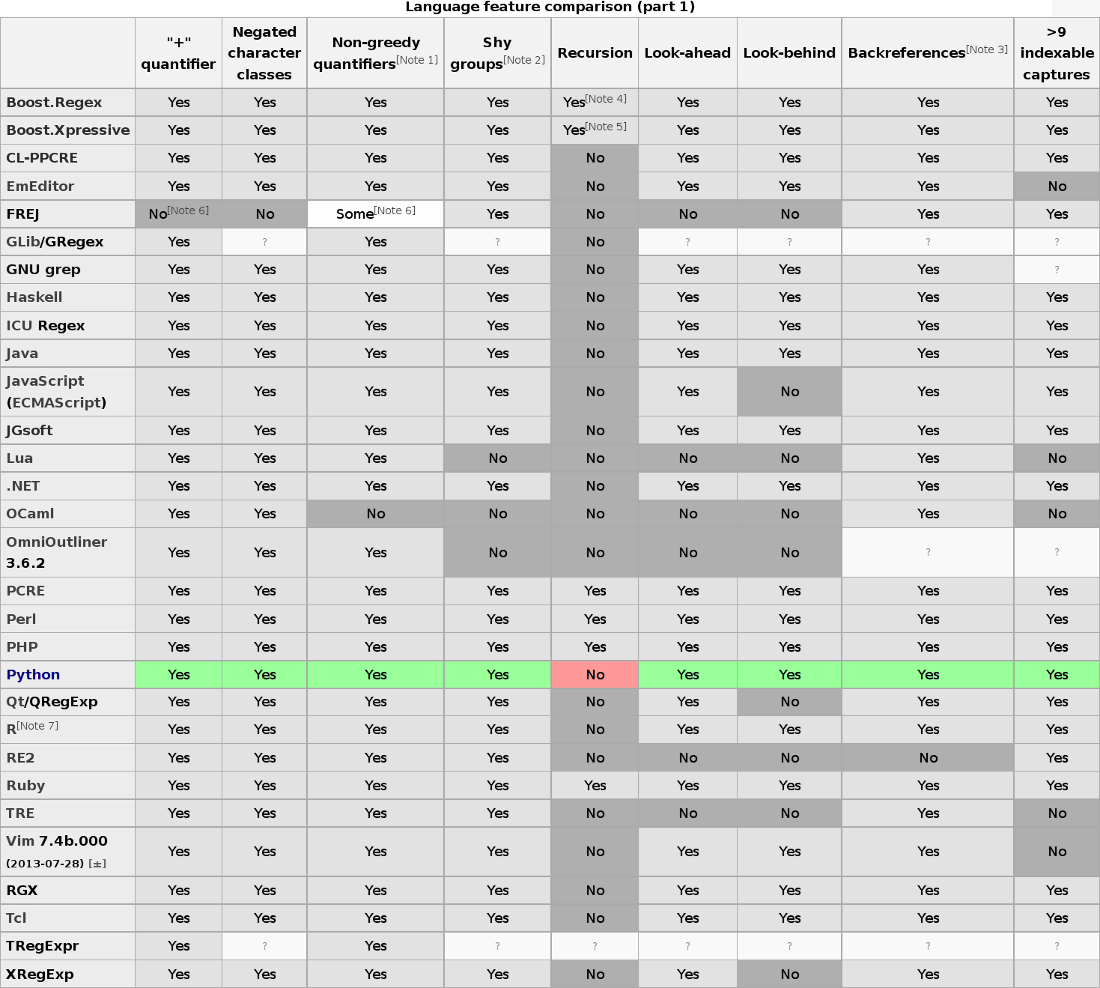
\includegraphics[width=0.70\textwidth]{images/re1.png}
\end{center}
\end{frame}

\begin{frame}
\begin{center}
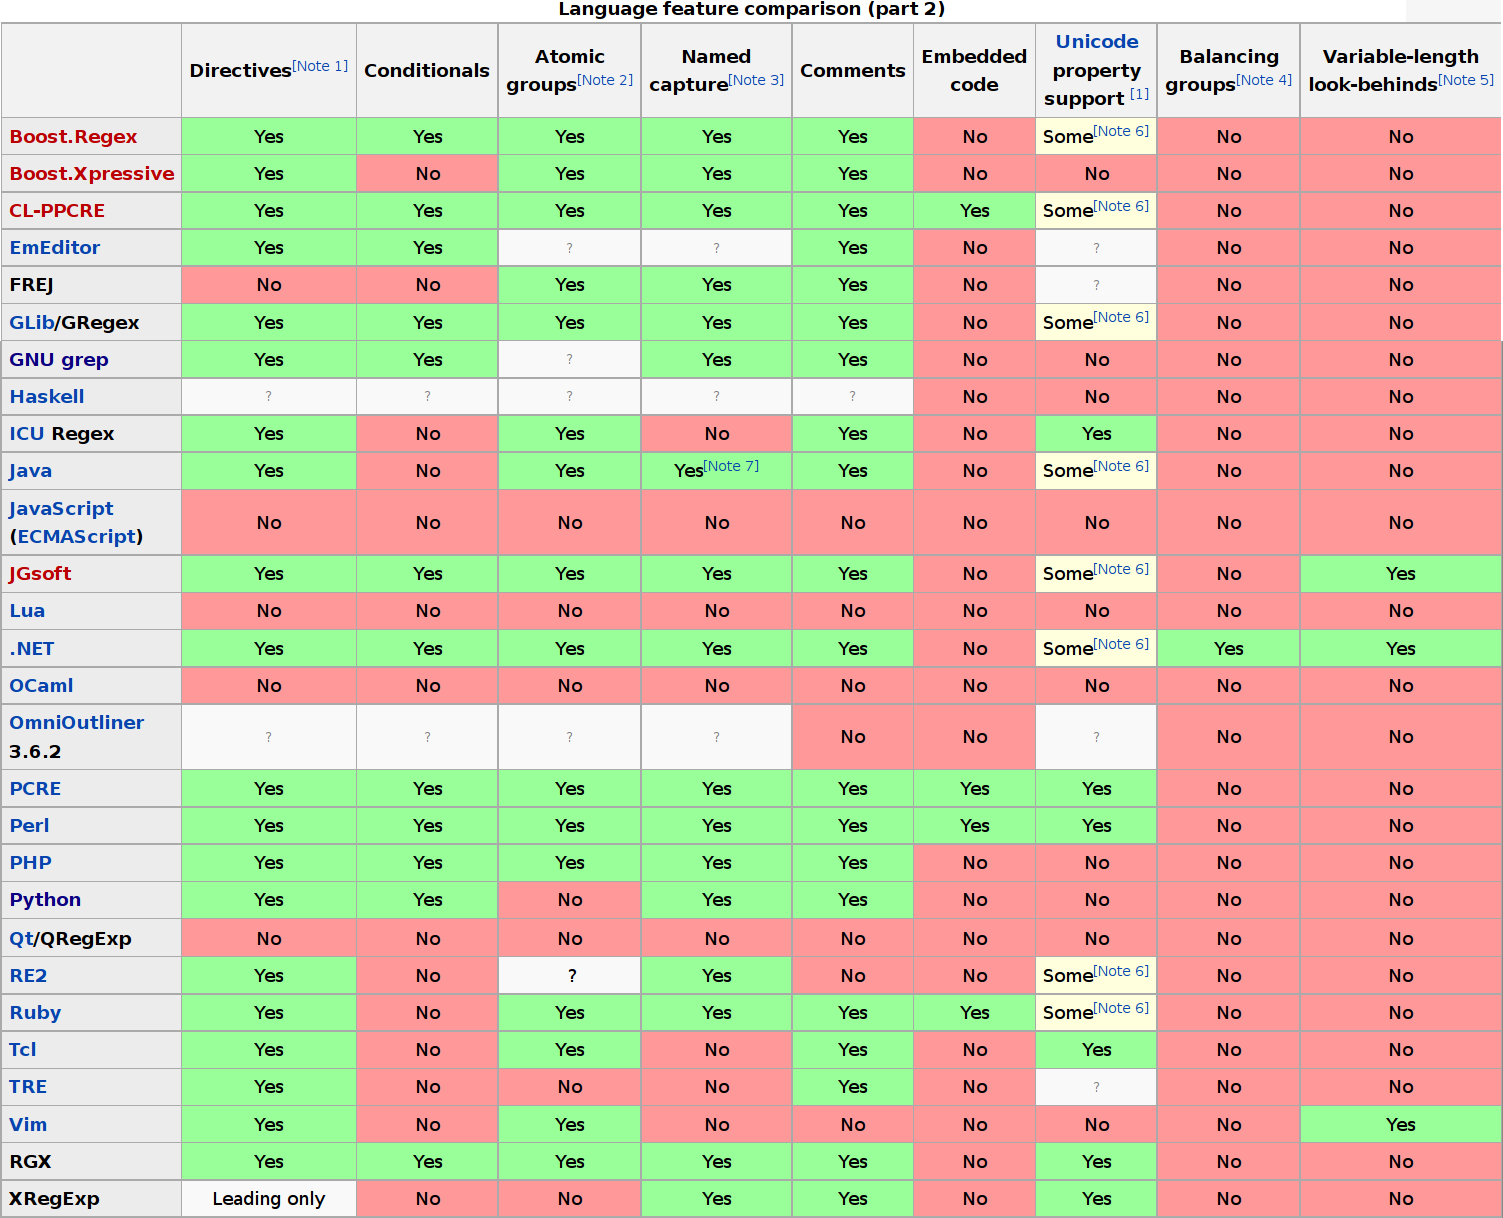
\includegraphics[width=0.70\textwidth]{images/re2.png}
\end{center}
\end{frame}

\section{Bibliography}
\begin{frame}
\begingroup
\fontsize{6pt}{8pt}\selectfont
\begin{itemize}
\item Regular Expression HOWTO: \url{https://docs.python.org/2/howto/regex.html}
\item Python Docs: Library re: \url{https://docs.python.org/2/library/re.html}
\item Google for Education. Python Regular Expressions: \url{https://developers.google.com/edu/python/regular-expressions?hl=en}
\item Regex Debugger: \url{https://regex101.com/}
\item Debuggex: \url{https://www.debuggex.com/}
\item Core Python Applications programming: Regular expressions: \url{http://www.informit.com/articles/article.aspx?p=1707750&seqNum=2}
\item Brief history by Staffan Noteberg: \url{http://blog.staffannoteberg.com/}
\end{itemize}
\endgroup
\end{frame}
\end{document}
